\documentclass{standalone}

\usepackage{tikz}
\usetikzlibrary{calc} % to compute rectangle coords on the fly
\usetikzlibrary{positioning} % for below of=
\usepackage{kpfonts}

\begin{document}

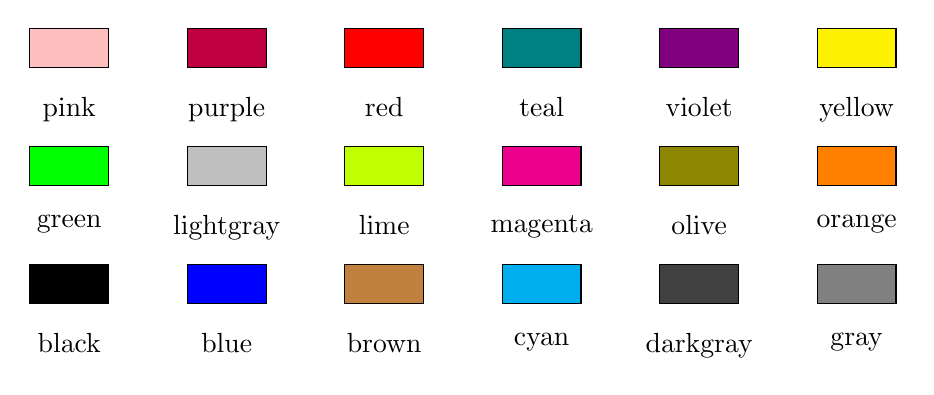
\begin{tikzpicture}
    \def \columnWidth {6};
    \def \baseWidth {0.5cm};
    \def \baseHeight {0.25cm};

    \foreach \color [count=\i from 0] in {black, blue, brown, cyan, darkgray, gray,
                                         green, lightgray, lime, magenta, olive,
                                         orange, pink, purple, red, teal, violet,
                                         yellow} {

        \coordinate (center_\color)
                        at ({2*mod(\i, \columnWidth)}, {1.5*div(\i, \columnWidth)});
        \coordinate (rectangle_bottom_\color)
                        at ($(center_\color) - (\baseWidth, \baseHeight)$);
        \coordinate (rectangle_top_\color)
                        at ($(center_\color) + (\baseWidth, \baseHeight)$);
        
        \draw[fill=\color, black] (rectangle_bottom_\color) rectangle (rectangle_top_\color);
        \node[below=0.5cm of center_\color] {\color};
    }
\end{tikzpicture}

\end{document}
